\documentclass[12pt,a4paper]{article}

% Margins.
\setlength{\oddsidemargin}{0in}
\setlength{\evensidemargin}{0in}
\setlength{\headheight}{12pt}
\setlength{\headsep}{42pt}
\setlength{\topmargin}{-70pt}
\setlength{\textwidth}{6.5in}
\setlength{\textheight}{10in}
\pagestyle{empty}

\usepackage{amsmath}
\usepackage{float}
\usepackage{graphicx}
\usepackage[hyphens]{url}
\usepackage[hidelinks]{hyperref}	% Clickable links to figures, references and urls.
\usepackage{lastpage}

% Drawing.
\usepackage{pgf}
\usepackage{tikz}

% Listings for formatting code.
\usepackage{listings}
\usepackage{textcomp}
% General options.
\lstset{breaklines=true, basicstyle=\footnotesize\ttfamily, tabsize=4, numbers=none, stepnumber=1, frame=single, showstringspaces=false, upquote=true}
% C++ specific high-lighting. Comments are 50/50 shades of green/black and strings coloured with 60/40 red/black mixture.
\lstset{language=[ISO]C++, commentstyle=\color{green!50!black}, keywordstyle=\color{blue}, stringstyle=\color{red!60!black}}

% Marks of each question.
\def\QOne{10}
\def\Qtwo{10}
\def\Qthree{10}
\def\Qfour{10}
\def\Qfive{10}
\def\TotalMarks{50}

\begin{document}
\begin{minipage}{0.55\textwidth}
{\LARGE \textbf{Physics for Engineers}}\\[0.15cm]
{\normalsize \textbf{Spring 2014 Semester}}\\
{\Large \textbf{$2^{nd}$ Sessional Exam}}\\
{\normalsize \textbf{Saturday, February 22, 2014}}\\[0.30cm]
{\Large \textbf{Total Time: 60 minutes}}\\[0.15cm]
{\Large \textbf{Total Marks: 50}}\\
\textbf{Course Instructor:}\\
Attique Dawood\\
\end{minipage}
\begin{minipage}{0.4\textwidth}
\textbf{Serial} \hrulefill \\[0.25cm]
\textbf{Name} \hrulefill\\[0.25cm]
\textbf{Section} \rule{1cm}{0.2mm} \textbf{Roll No:} \hrulefill\\[0.25cm]
\textbf{Signature:} \hrulefill\\[0.25cm]
\rule{6.6cm}{0.2mm}\\
\textbf{Signature of Invigilator}\\[0.25cm]
\end{minipage}
\begin{table}[H]
\begin{center}
\vspace{0.3cm}
	{\large \begin{tabular}{|l|c|c|c|c|c|c|}
	\hline
		\rule{0pt}{2.6ex} Question & \textbf{1} & \textbf{2} & \textbf{3} & \textbf{4} & \textbf{5} & \textbf{Total}\\
		\hline
		Marks Obtained \rule{0pt}{2.6ex} & & & & & &\\
		\hline
		Total Marks \rule{0pt}{2.6ex} & \QOne & \Qtwo & \Qthree & \Qfour & \Qfive & \TotalMarks\\		
	\hline
	\end{tabular}}
\end{center}
\end{table}
\noindent \textbf{You are advised to READ these notes:}
\begin{enumerate}
\item \textbf{Attempt on the Question Paper. \underline{NO EXTRA SHEET} will be provided/accepted. No
additional sheet will be provided for rough work. Use the back of the page where
provided space is not sufficient.}
\item After asked to commence the exam, please verify that you have \textbf{\pageref{LastPage} different
printed pages} including this title page.
\item There are 5 questions. Attempt all of them. It is advisable to go through the paper once
before starting with the first question.
\item Exam is closed books, closed notes. Please see that the area in your threshold is clean.
You will be charged for any material which can be classified as \textbf{`helping in the paper'}
found near you.
\item \textbf{Calculator sharing is strictly prohibited.}
\item Students who attempt the paper with lead pencils lose the right to get them rechecked.
\item \textbf{The invigilator present is not supposed to answer any questions. No one may come
to your room for corrections and you are not supposed to request to call anyone.
Make assumptions wherever required and clearly mark them.}
\end{enumerate}
\newpage
\noindent\textbf{Question 1: Coordinate Conversion\hfill \QOne~marks}\\
Convert the point P(-1, 2, -3) to cylindrical and spherical coordinates.
\newpage

\noindent \textbf{Question 2: Vector Fields and Vector Field Conversion\hfill \Qtwo~marks}\\
A vector field is given by $\textbf{A}=(1-yz)\hat x+(x+y)\hat y+z^3\hat z$. What is the cylindrical coordinates representation of this vector field at (-2, 1, 1). Also find the magnitude at (-2, 1, 1). Magnitude can be found from either cartesian or cylindrical representation. Unit vector conversions are
\begin{equation*}
\begin{split}
&\hat x=\cos\phi\hat \rho-\sin\phi \hat \phi\\
&\hat y=\sin\phi\hat \rho+\cos\phi \hat \phi\\
\end{split}
\end{equation*}
\newpage

\noindent\textbf{Question 3: Volume Integral \hfill \Qthree~marks}\\
Find the total mass of a spherical rock of radius 1 m and mass density $\rho_m=\dfrac{3}{4\pi r}$ kg/m$^3$.
\newpage

\noindent\textbf{Question 4: Flux of a Vector Field \hfill \Qfour~marks}\\
Vector field in a region is $\textbf{A}=(z-yx)\hat x+(x+y)\hat y+z^3\hat z$. Evaluate the flux, $\int\limits_{S}\textbf{A}\cdot d\textbf{S}$, through the surface given by $x=-2$, $0<y<2$ and $-1<z<2$.
\newpage

\noindent\textbf{Question 5: Line Integral \hfill \Qfive~marks}\\
Force field in a region is $\textbf{F}=y^2\hat x+2xy\hat y$ find the work done in moving from A to C along
\begin{itemize}
\item[a.] Path ABC.
\item[b.] Direct path AC.
\end{itemize}
Formula for work done is $W_{AC}=\int\limits_{A}^{C} \textbf{F}\cdot d\textbf{\textit{l}}$.
\begin{figure}[H]
\flushright
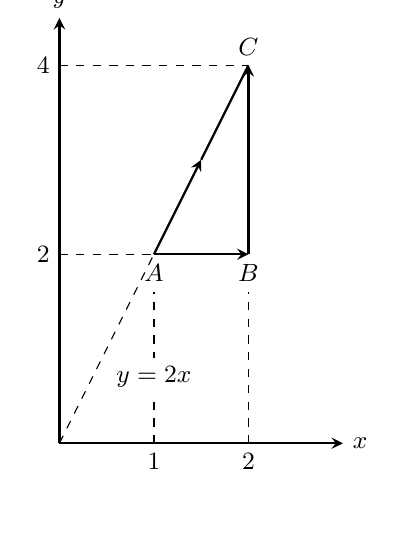
\begin{tikzpicture}[xscale=1.2,yscale=1.2,font=\small]
	\def\XD{0cm}
	\def\YD{0cm}

	\draw[thick, ->, >=stealth] (1cm, 2cm) -- (2cm, 2cm);
	\draw[thick, ->, >=stealth] (2cm, 2cm) -- (2cm, 4cm);
	%\draw[thick, ->, >=stealth] (2cm, 4cm) -- (1cm, 4cm);
	%\draw[thick, ->, >=stealth] (1cm, 4cm) -- (1cm, 2cm);
	\draw[thick, ->, >=stealth] (1cm, 2cm) -- (1.5cm, 3cm);
	\draw[thick] (1.5cm, 3cm) -- (2cm, 4cm);

	\draw[dashed] (0cm, 0cm) -- (1cm, 2cm);
	\draw[dashed] (0cm, 2cm) -- (1cm, 2cm);
	\draw[dashed] (0cm, 4cm) -- (2cm, 4cm);
	\draw[dashed] (1cm, 0cm) -- (1cm, 1.6cm);
	\draw[dashed] (2cm, 0cm) -- (2cm, 1.6cm);
	\draw[white,fill=white] (0.5cm,0.5cm) rectangle (1.5cm, 0.9cm);
	\node at (1cm, 0.7cm){$y=2x$};

	\coordinate[label=above:$C$] (C) at (2cm,4cm);
	%\coordinate[label=above:$D$] (D) at (1cm,4cm);
	\coordinate[label=below:$A$] (A) at (1cm,2cm);
	\coordinate[label=below:$B$] (B) at (2cm,2cm);
	
	\coordinate[label=left:$2$] (y1) at (0cm,2cm);
	\coordinate[label=left:$4$] (y2) at (0cm,4cm);
	\coordinate[label=below:$1$] (x1) at (1cm,0cm);
	\coordinate[label=below:$2$] (x2) at (2cm,0cm);
	
	\draw[thick, ->, >=stealth] (0cm, 0cm) -- (0cm, 4.5cm);
	\coordinate[label=above:$y$] (y) at (0cm,4.5cm);
	\draw[thick, ->, >=stealth] (0cm, 0cm) -- (3cm, 0cm);
	\coordinate[label=right:$x$] (x) at (3cm,0cm);

\end{tikzpicture}
\end{figure}

\end{document}